\documentclass[conference]{IEEEtran}

\usepackage{cite}
\usepackage{graphicx}
\usepackage{amsmath}
\usepackage{booktabs}
\usepackage{url}
\usepackage{hyperref}

\begin{document}

\title{Spatio-Temporal Crime Occurrence Prediction and Crime Type Forecasting in Chicago Using Interpretable Machine Learning}

\author{
\IEEEauthorblockN{Dilip Thakur}
\IEEEauthorblockA{
University of St. Thomas\\
Saint Paul, Minnesota, USA\\
Email: your-email-here
}
}

\maketitle

\begin{abstract}
Urban crime forecasting is a challenging spatio-temporal prediction problem because crime patterns vary across both location and time. This study uses reported crime incidents from the Chicago Crime Dataset between January 1, 2024 and December 31, 2025 to develop two predictive tasks: crime occurrence prediction and grouped crime type forecasting. The original event-only dataset was transformed into a supervised Community Area by Hour dataset, producing approximately 1.35 million hourly observations with both crime and no-crime examples. Temporal, cyclical, lag-based, and rolling-window features were engineered to capture short-term crime patterns. Logistic Regression, Random Forest, Histogram Gradient Boosting, and a Neural Network MLP were evaluated using a chronological non-shuffled train-test split. For crime occurrence prediction, Histogram Gradient Boosting achieved the strongest threshold-tuned F1-score of 0.525, while Random Forest achieved the highest recall of 0.629. For grouped crime type forecasting, Random Forest achieved the best balanced performance with a Macro-F1 score of 0.400. Results show that crime occurrence prediction is more reliable than grouped crime type forecasting using only spatial and temporal features. The study also discusses limitations related to reported-crime bias, missing external context, and responsible use of predictive models in public-safety settings.
\end{abstract}

\begin{IEEEkeywords}
crime prediction, spatio-temporal forecasting, machine learning, Chicago crime data, interpretable machine learning, public safety analytics
\end{IEEEkeywords}

\section{Introduction}

Urban crime analysis is an important application area for data science because crime patterns often vary across location, time of day, day of week, and neighborhood context. Public crime datasets provide an opportunity to study these patterns using machine learning methods. However, crime forecasting is difficult because reported crime incidents are sparse, imbalanced, and affected by social, spatial, and reporting factors.

This study focuses on short-term crime forecasting in Chicago using public crime records from the Chicago Data Portal. The work is organized around two prediction tasks. The first task is crime occurrence prediction, where the goal is to predict whether at least one crime will occur in a given Chicago community area during a given hour. The second task is grouped crime type forecasting, where the goal is to predict the broader category of crime once a crime occurrence exists.

A key challenge is that the original dataset contains only reported crime events. It does not directly contain no-crime examples. To address this, the event-level data is converted into a complete Community Area by Hour grid. This creates a supervised learning dataset containing both crime and no-crime observations. The resulting dataset allows binary crime occurrence prediction while preserving spatial and temporal structure.

The main contribution of this work is not a new deep learning architecture. Instead, this paper presents a reproducible empirical pipeline for transforming event-only crime records into a supervised spatio-temporal forecasting dataset and comparing multiple model families under a chronological non-shuffled evaluation setup.

The main contributions are:
\begin{itemize}
    \item A Community Area by Hour supervised dataset construction from event-only Chicago crime records.
    \item Temporal, cyclical, lag-based, and rolling-window feature engineering for short-term crime forecasting.
    \item A comparison of Logistic Regression, Random Forest, Histogram Gradient Boosting, and Neural Network MLP models.
    \item Separate evaluation of crime occurrence prediction and grouped crime type forecasting.
    \item Discussion of interpretability, limitations, and ethical concerns related to predictive crime modeling.
\end{itemize}

\section{Related Work}

Crime prediction has often been studied as a spatio-temporal forecasting problem, where historical crime records are aggregated over spatial regions and time intervals to estimate future crime risk. Prior studies have explored statistical models, machine learning models, deep learning architectures, and graph-based approaches for this task.

Recent work has applied advanced spatio-temporal deep learning methods to urban crime forecasting, including graph convolutional networks, recurrent neural networks, and transformer-style temporal models. Some studies have specifically used Chicago crime data due to its public availability and detailed spatial attributes. Compared with these methods, this study emphasizes a simpler and reproducible machine learning pipeline rather than a complex neural architecture.

Interpretability is also important in crime prediction because public-safety models can affect sensitive decisions. Prior work has used feature importance and SHAP-based explanations to analyze machine learning predictions. This study follows the same general direction by including feature-importance analysis for the best-performing tree-based models.

Crime prediction also raises ethical concerns. Reported crime datasets do not represent all crime; they represent incidents that were reported, recorded, and processed. As a result, such data may reflect reporting bias, enforcement bias, and unequal policing patterns. This study treats crime forecasting as an aggregate academic analysis task and does not propose direct use for individual-level policing decisions.

\section{Dataset and Preprocessing}

The dataset used in this study is the Chicago Crime Dataset from the Chicago Data Portal. Records were filtered from January 1, 2024 to December 31, 2025. The raw dataset contained approximately 494,273 crime incident records and 22 attributes, including date, location, community area, district, primary crime type, arrest status, domestic flag, latitude, and longitude.

Records with missing geographic coordinates were removed, leaving approximately 492,776 usable records. The date column was converted into a timestamp, and additional temporal fields such as hour, day of week, month, day, and weekend indicator were extracted.

For crime occurrence prediction, the original event-level data was transformed into a complete Community Area by Hour grid. Each row represents one Chicago community area during one hour. The target variable indicates whether at least one crime occurred in that community area and hour. This process produced 1,352,736 hourly observations.

For crime type forecasting, original crime types were grouped into broader categories: Property, Violent, and Other. Rows with no crime occurrence were excluded from this task because crime type is only defined when a crime occurred.

\section{Feature Engineering}

The feature set was designed to capture spatial, temporal, and recent historical crime patterns. Spatial information was represented using community area. Temporal information included hour, day of week, month, day, and weekend indicator.

To represent the cyclical nature of time, hour was encoded using sine and cosine transformations. This avoids treating hour 23 and hour 0 as far apart when they are actually adjacent in daily time.

Lag features were created to represent recent crime activity in the same community area. These included one-hour, two-hour, three-hour, and twenty-four-hour lag values. Rolling mean features were also created using three-hour, six-hour, twelve-hour, and twenty-four-hour windows.

These features were used to help the models learn whether recent crime patterns were associated with future crime occurrence or crime type.

\section{Methodology}

A chronological non-shuffled train-test split was used. This is important because random splitting can leak future temporal patterns into the training data. The first 80\% of time periods were used for training, and the remaining 20\% were used for testing.

Four model families were evaluated:
\begin{itemize}
    \item Logistic Regression
    \item Random Forest
    \item Histogram Gradient Boosting
    \item Neural Network MLP
\end{itemize}

For crime occurrence prediction, the task was treated as binary classification. The evaluation metrics included accuracy, precision, recall, F1-score, ROC-AUC, PR-AUC, and threshold-tuned F1-score.

For grouped crime type forecasting, the task was treated as multiclass classification. The evaluation metrics included accuracy, Macro-F1, and Weighted-F1. Macro-F1 was emphasized because it gives equal weight to all classes and is more informative when class imbalance exists.

\section{Experimental Results}

\subsection{Crime Occurrence Prediction}

Crime occurrence prediction produced stronger results than crime type forecasting. Histogram Gradient Boosting achieved the highest accuracy, ROC-AUC, PR-AUC, and threshold-tuned F1-score. It achieved an accuracy of 0.7675, ROC-AUC of 0.7484, PR-AUC of 0.5160, and best threshold F1-score of 0.5246 at a threshold of 0.27.

Random Forest achieved the highest recall of 0.6288 and the strongest default-threshold F1-score of 0.5128. This suggests that Random Forest may be useful when the goal is to capture more potential crime-occurrence cases, while Histogram Gradient Boosting provides stronger overall ranking and threshold-tuned performance.

\begin{table}[htbp]
\caption{Crime Occurrence Prediction Results}
\centering
\resizebox{\linewidth}{!}{
\begin{tabular}{lcccccc}
\toprule
Model & Accuracy & Precision & Recall & F1 & ROC-AUC & PR-AUC \\
\midrule
Random Forest & 0.693 & 0.433 & 0.629 & 0.513 & 0.737 & 0.505 \\
Logistic Regression & 0.704 & 0.441 & 0.568 & 0.496 & 0.721 & 0.483 \\
Hist. Gradient Boosting & 0.767 & 0.607 & 0.266 & 0.370 & 0.748 & 0.516 \\
Neural Network MLP & 0.764 & 0.607 & 0.231 & 0.335 & 0.733 & 0.499 \\
\bottomrule
\end{tabular}
}
\label{tab:occurrence_results}
\end{table}

\begin{figure}[htbp]
\centerline{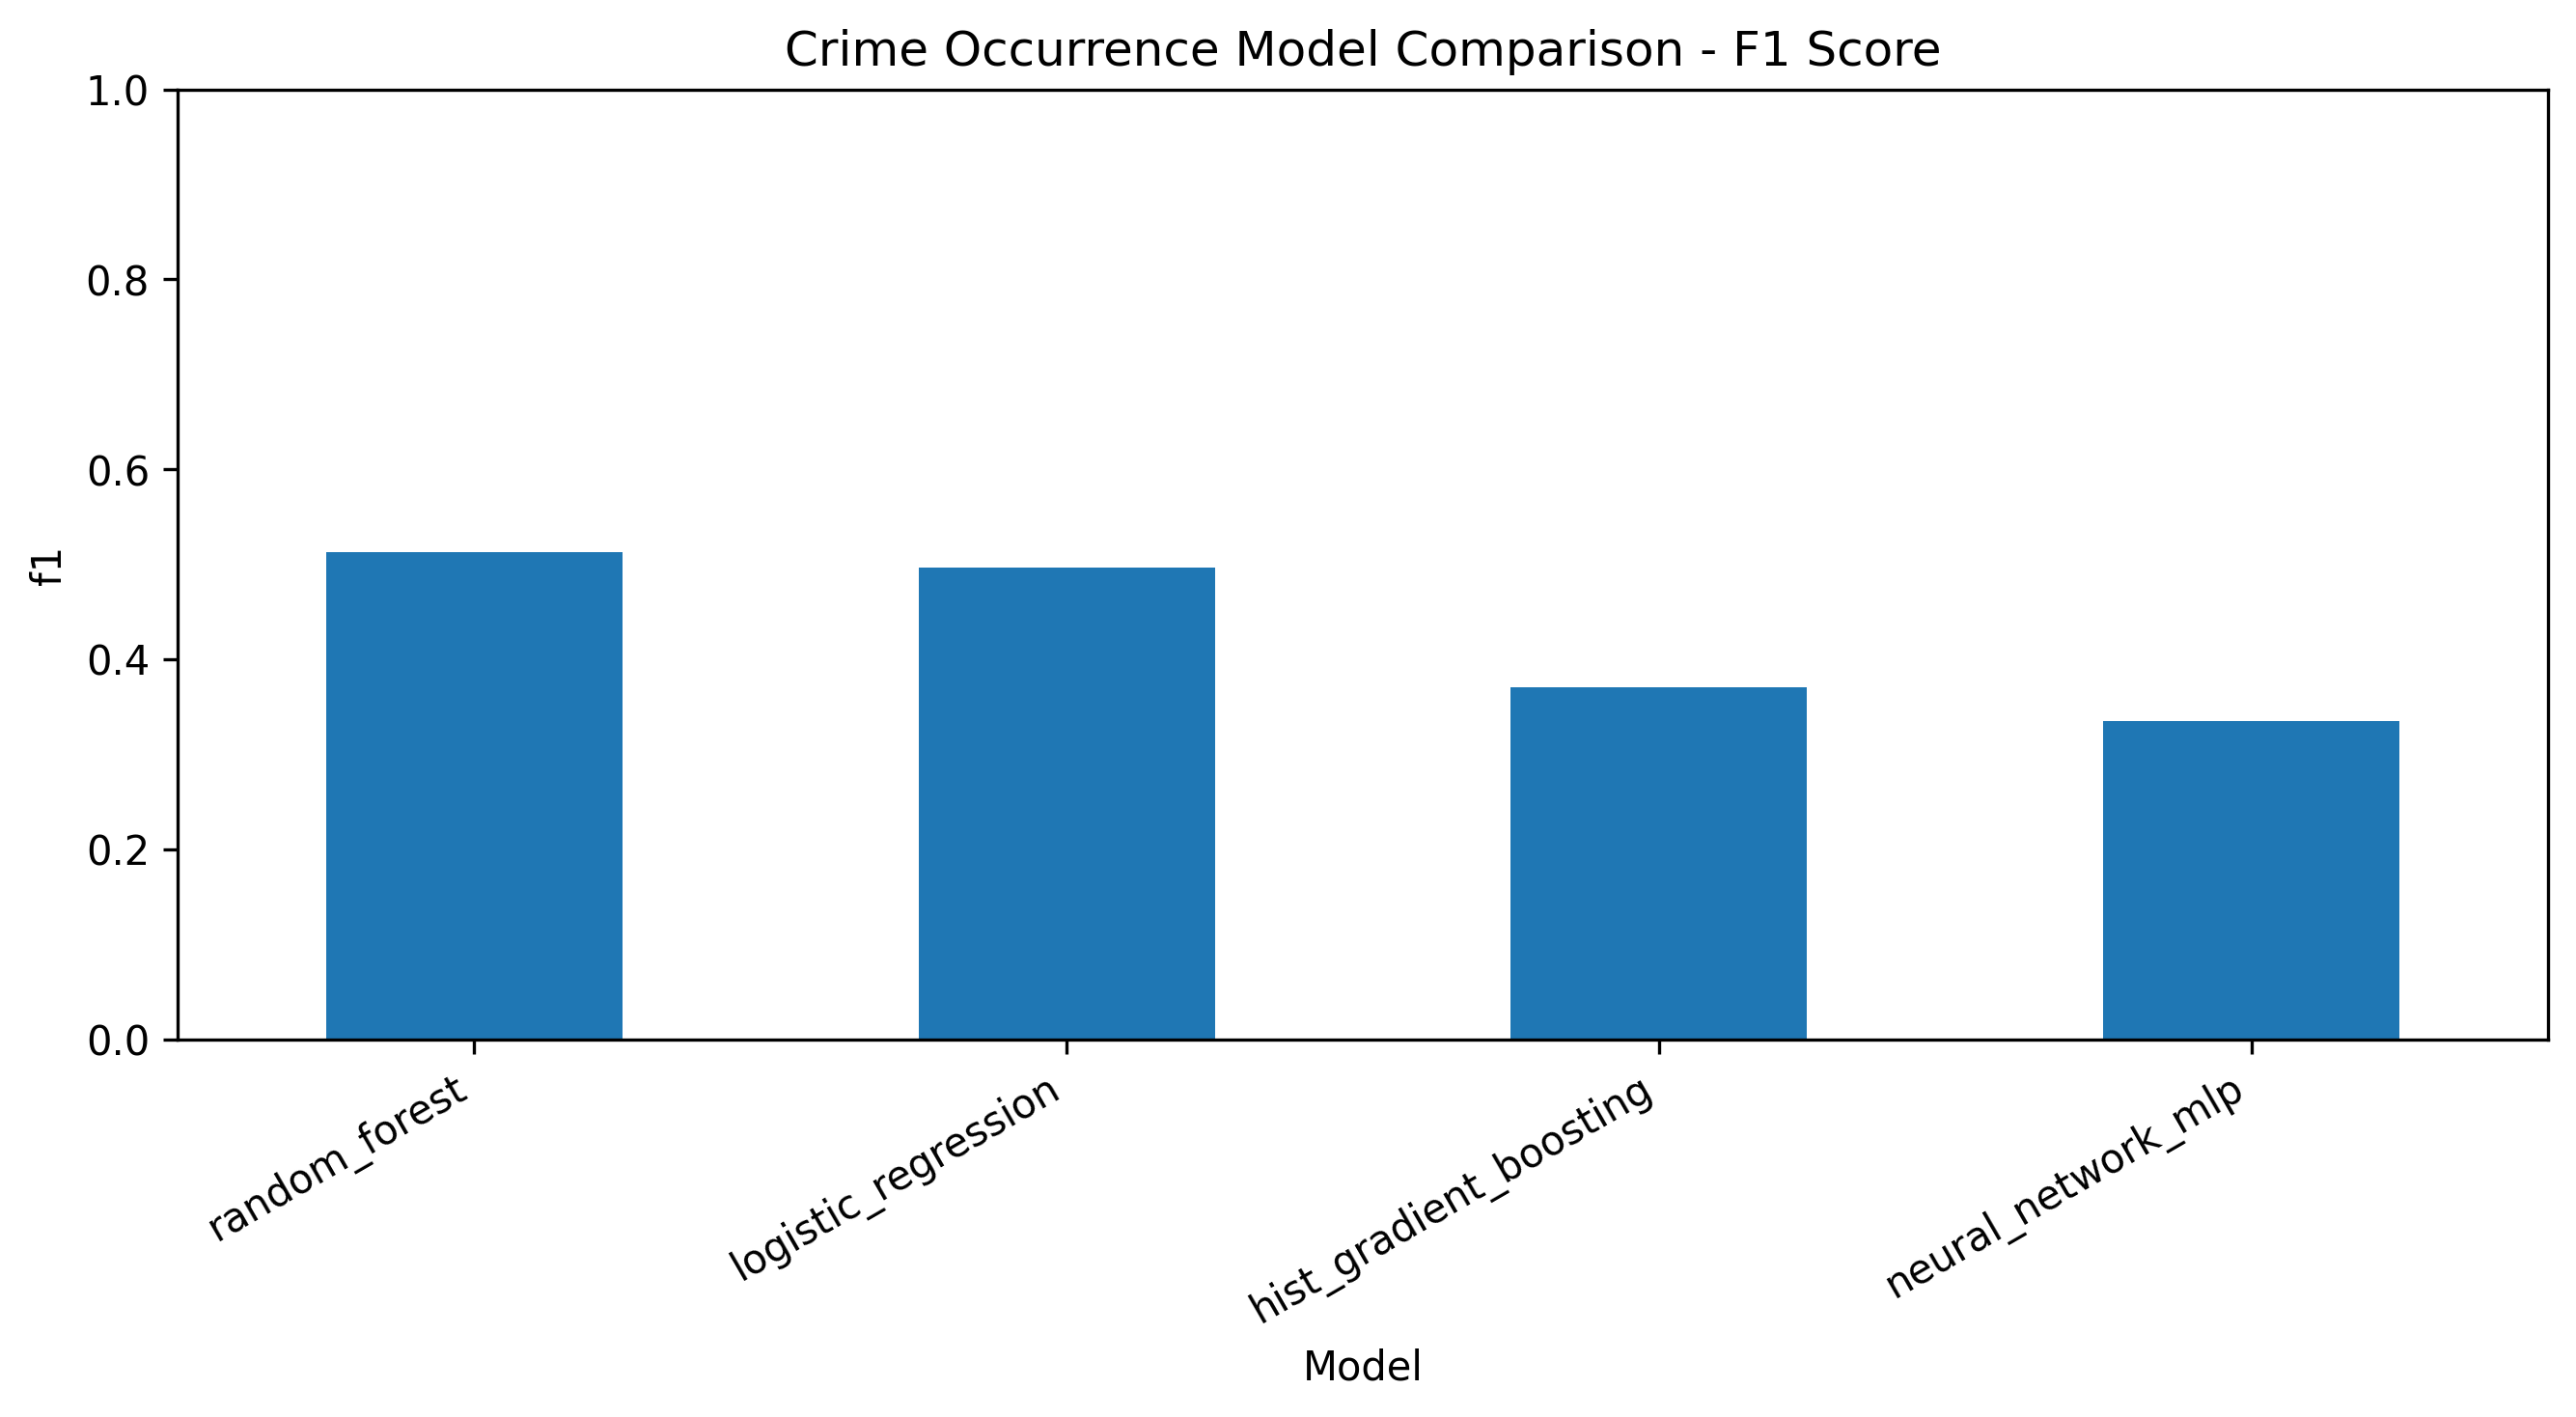
\includegraphics[width=\linewidth]{figures/occurrence_model_comparison_f1.png}}
\caption{F1-score comparison for crime occurrence prediction models.}
\label{fig:occurrence_f1}
\end{figure}

\begin{figure}[htbp]
\centerline{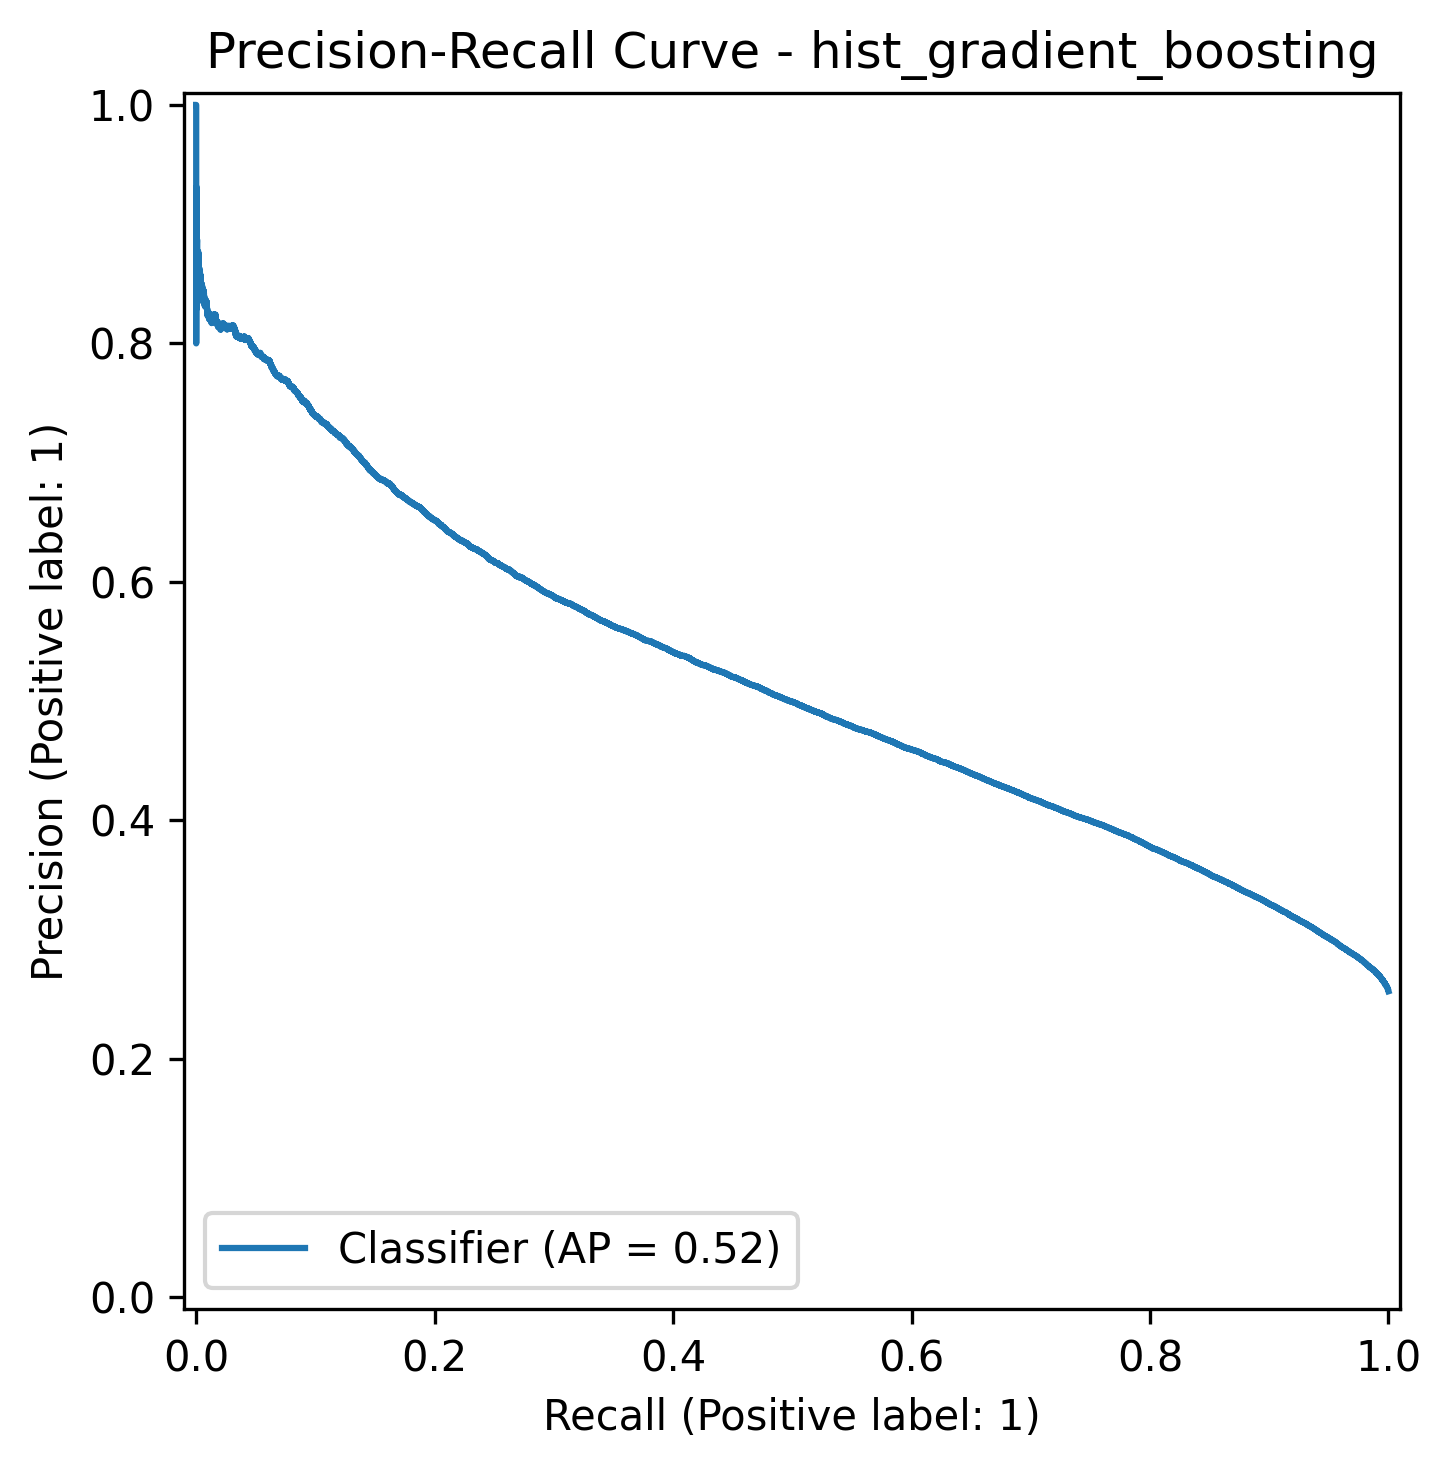
\includegraphics[width=\linewidth]{figures/occurrence_hist_gradient_boosting_pr_curve.png}}
\caption{Precision-recall curve for Histogram Gradient Boosting on crime occurrence prediction.}
\label{fig:occurrence_pr}
\end{figure}

\subsection{Grouped Crime Type Forecasting}

Grouped crime type forecasting was more difficult. Random Forest achieved the best balanced performance, with an accuracy of 0.4389, Macro-F1 of 0.4004, and Weighted-F1 of 0.4578.

Histogram Gradient Boosting achieved the highest accuracy of 0.5699, but its Macro-F1 was only 0.2728. This suggests that the model may have favored the majority class. Therefore, Random Forest was considered the best balanced model for grouped crime type forecasting.

\begin{table}[htbp]
\caption{Grouped Crime Type Forecasting Results}
\centering
\resizebox{\linewidth}{!}{
\begin{tabular}{lccc}
\toprule
Model & Accuracy & Macro-F1 & Weighted-F1 \\
\midrule
Random Forest & 0.439 & 0.400 & 0.458 \\
Logistic Regression & 0.438 & 0.369 & 0.446 \\
Hist. Gradient Boosting & 0.570 & 0.273 & 0.434 \\
Neural Network MLP & 0.569 & 0.247 & 0.417 \\
\bottomrule
\end{tabular}
}
\label{tab:crime_type_results}
\end{table}

\begin{figure}[htbp]
\centerline{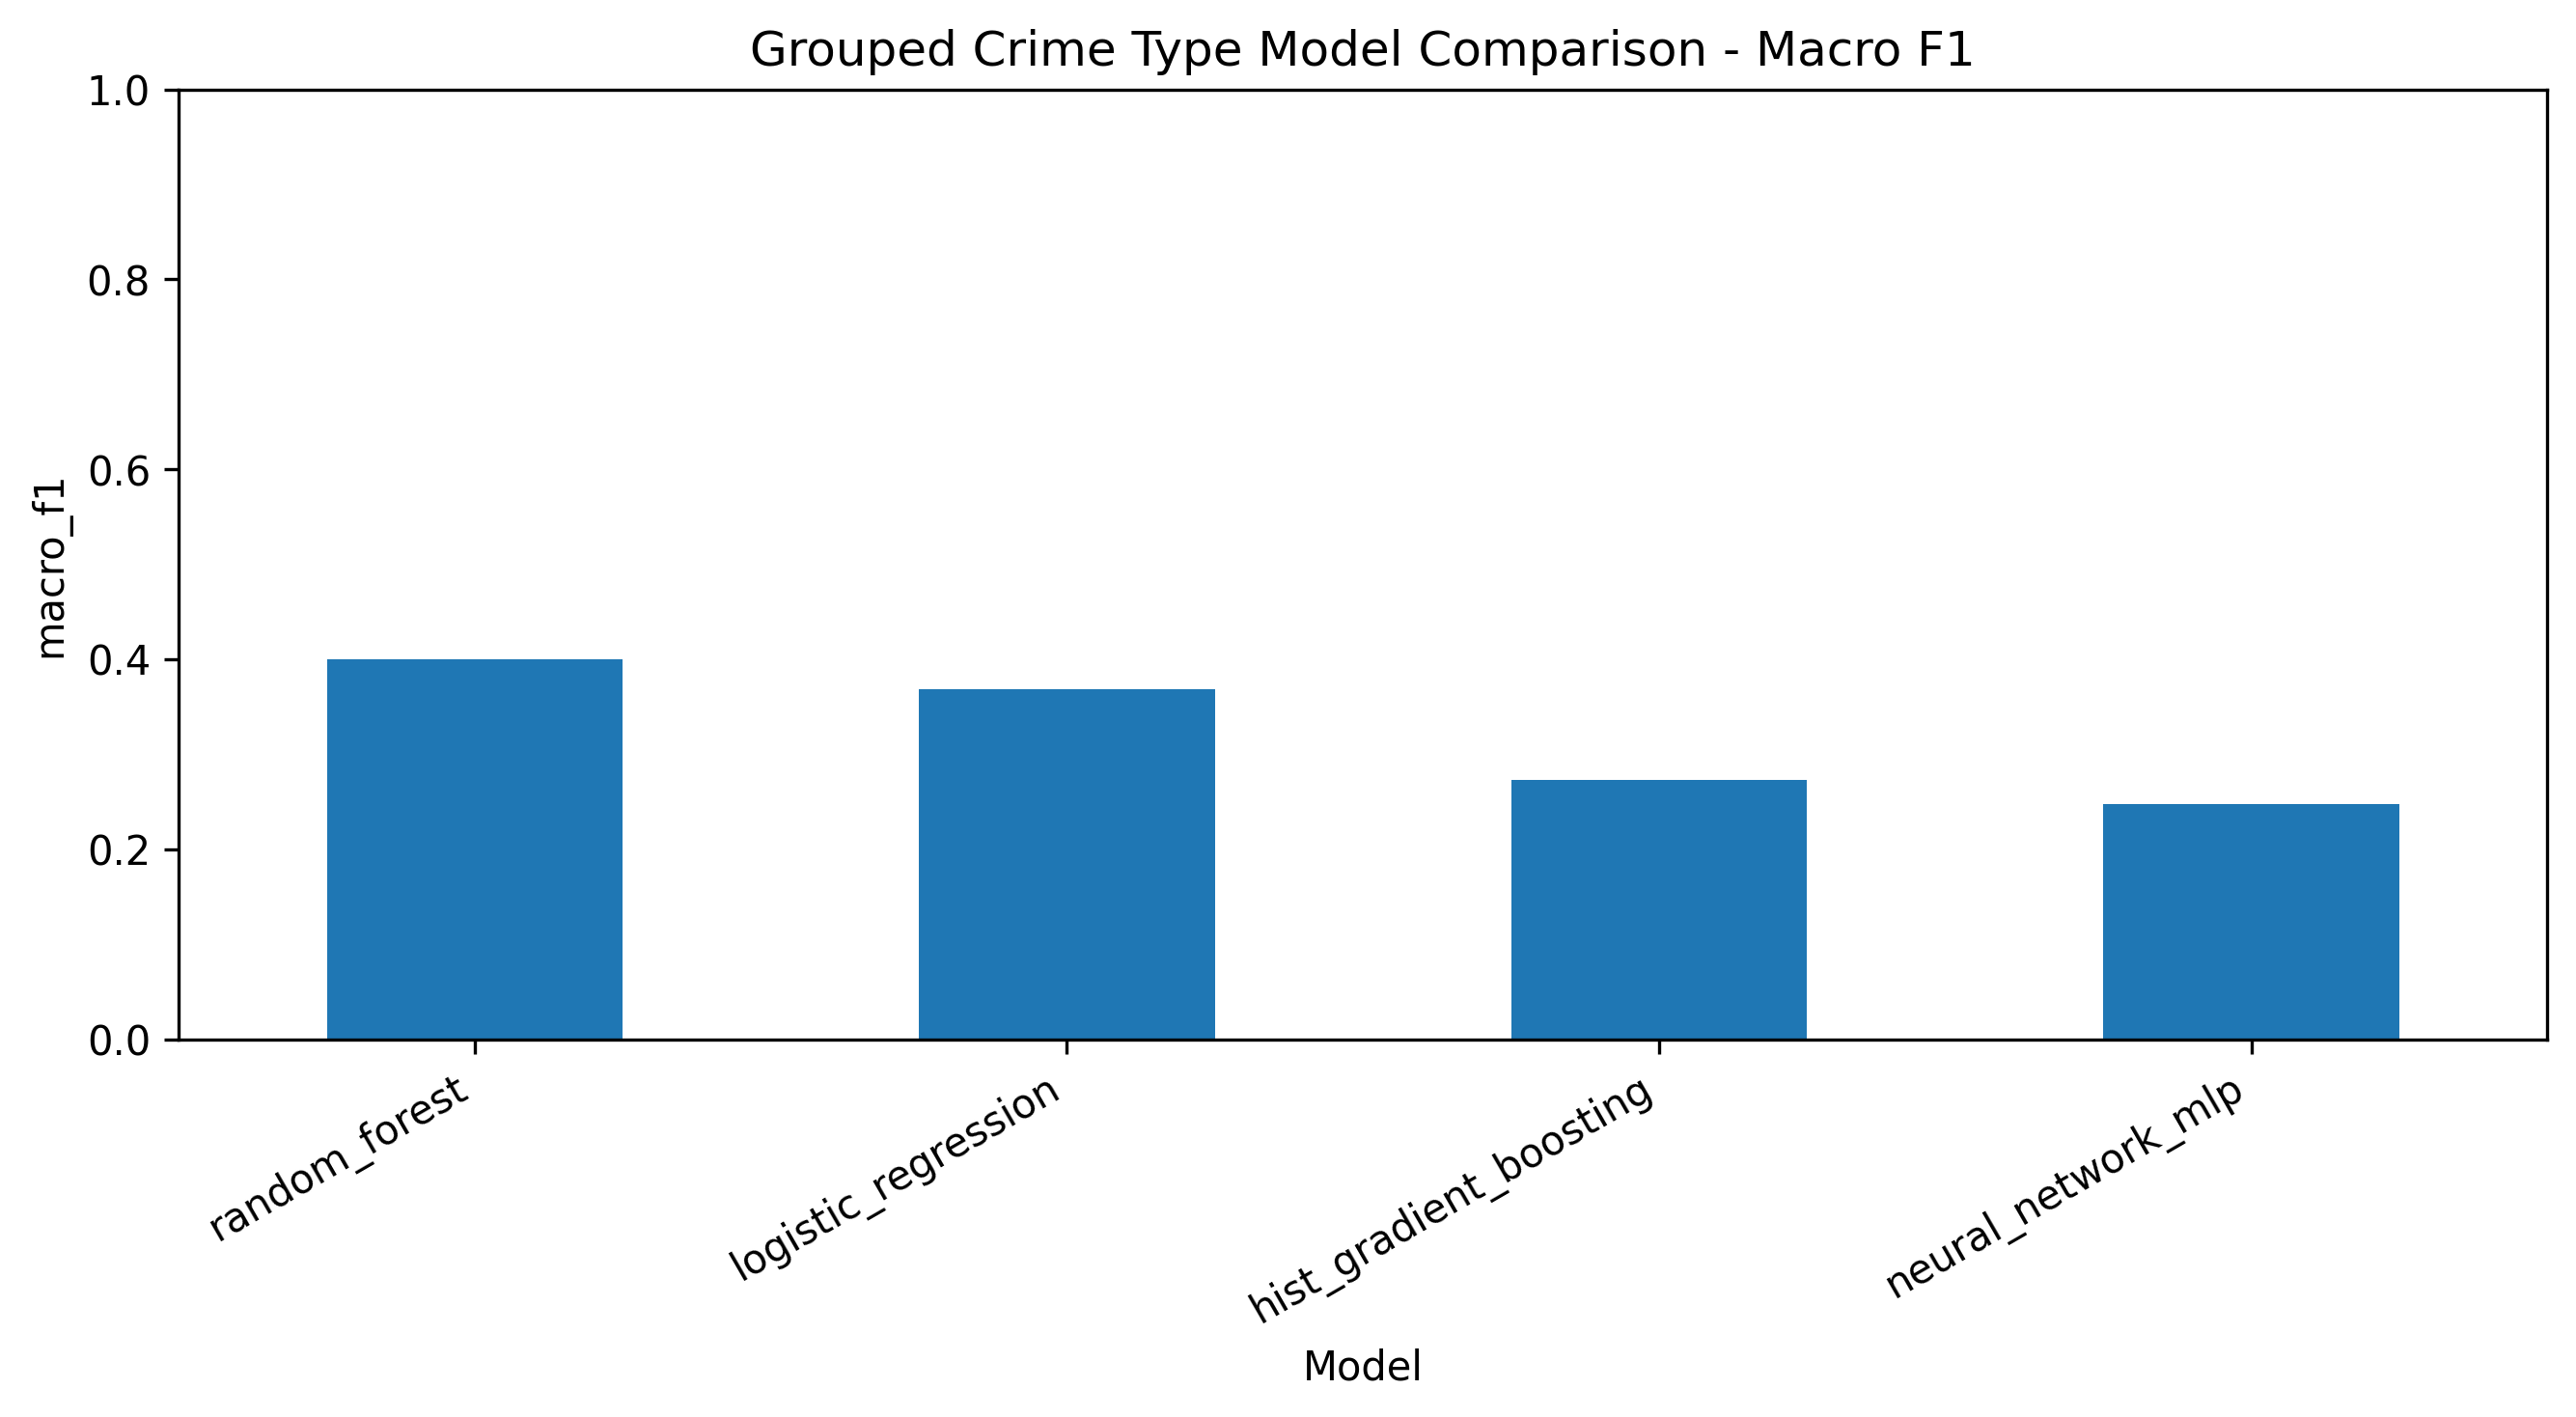
\includegraphics[width=\linewidth]{figures/crime_type_model_comparison_macro_f1.png}}
\caption{Macro-F1 comparison for grouped crime type forecasting models.}
\label{fig:crime_type_macro_f1}
\end{figure}

\begin{figure}[htbp]
\centerline{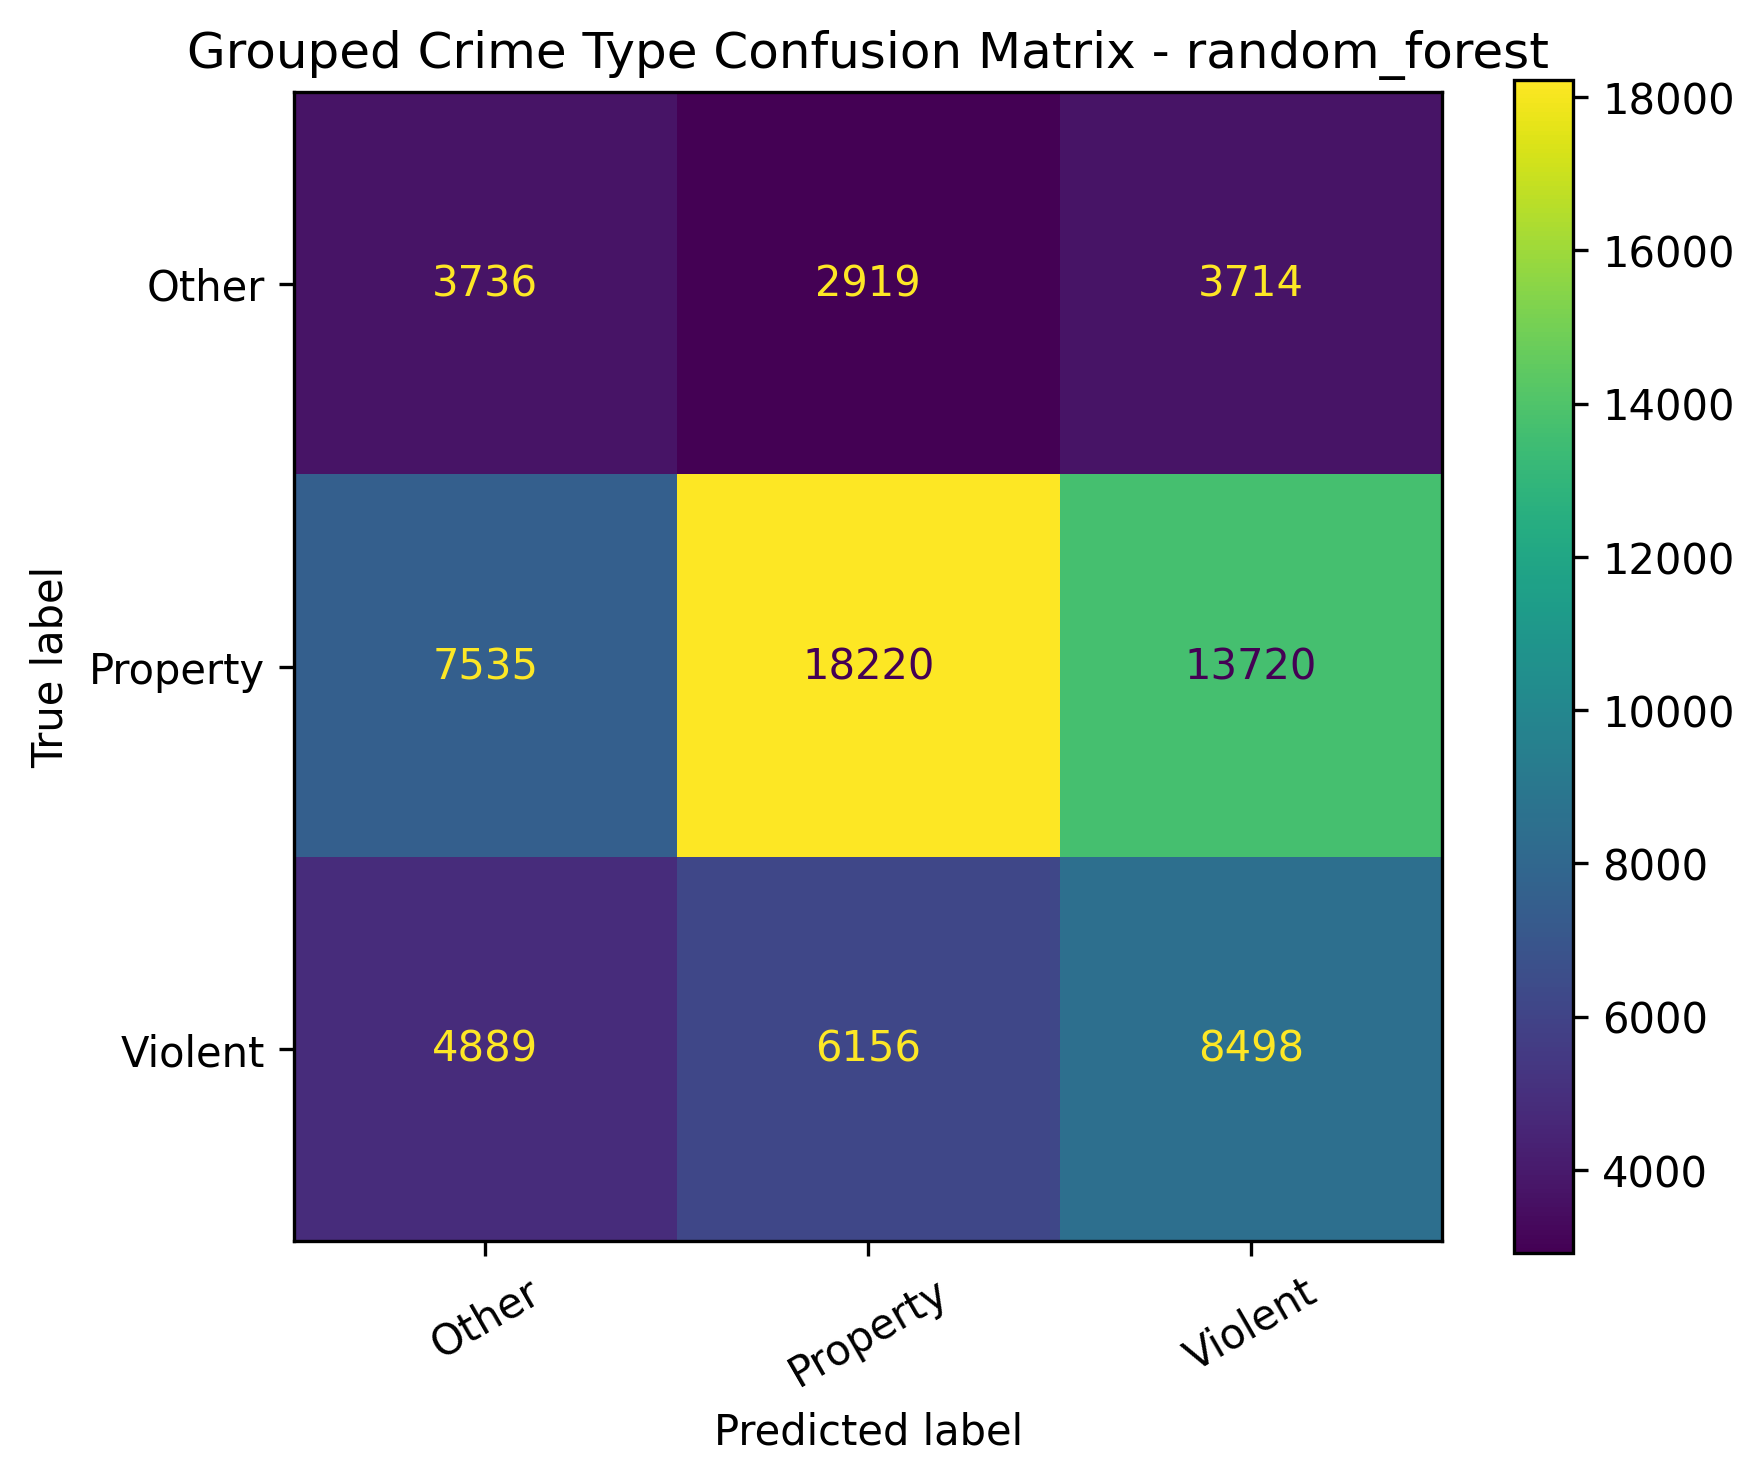
\includegraphics[width=\linewidth]{figures/crime_type_random_forest_confusion_matrix.png}}
\caption{Confusion matrix for Random Forest grouped crime type forecasting.}
\label{fig:crime_type_confusion}
\end{figure}

\section{Limitations and Ethical Considerations}

This study has several limitations. First, the dataset contains reported crime incidents, not all crimes that occurred. Some crimes may be underreported, while others may be more visible due to policing patterns, neighborhood conditions, or reporting behavior. Therefore, the model learns patterns in recorded incidents rather than true underlying crime occurrence.

Second, the model uses Chicago community areas as spatial units. This improves interpretability but hides smaller block-level differences within each community area. Third, the model uses spatial and temporal features, lag features, and rolling-window features, but it does not include external context such as weather, public events, holidays, school schedules, transit activity, population density, demographics, points of interest, or police deployment patterns.

Ethically, crime prediction must be handled carefully because models trained on historical crime data can reproduce or amplify existing biases. This work is intended only as an academic aggregate-level forecasting study. It should not be used for individual-level policing decisions, surveillance, or automated public-safety deployment. Any real-world use would require fairness testing, transparency, privacy safeguards, human oversight, and community review.

\section{Conclusion and Future Work}

This paper presented a reproducible machine learning pipeline for spatio-temporal crime occurrence prediction and grouped crime type forecasting using Chicago crime data. The original event-level data was transformed into a Community Area by Hour supervised learning dataset, allowing both crime and no-crime observations to be modeled.

The results show that crime occurrence prediction is more reliable than grouped crime type forecasting using the current feature set. Histogram Gradient Boosting achieved the best threshold-tuned F1-score for occurrence prediction, while Random Forest achieved the best balanced performance for grouped crime type forecasting.

Future work should incorporate richer external context such as weather, public events, holidays, demographics, population density, mobility patterns, and points of interest. Future research could also compare graph-based and sequence-based deep learning architectures under the same chronological evaluation setup.

\bibliographystyle{IEEEtran}
\bibliography{references}

\end{document}